\documentclass[french]{template}

\usepackage{textalpha} % Pour les mots grecs
\usepackage{minted} % Pour le code

\definecolor{LightGray}{gray}{0.9}

\begin{document}
\titre{Projet Immorthon}
\UE{Apprentissage Profond}
\enseignant{Axel \textsc{Carlier}}

\eleves{Axel \textsc{Bechu} \\ Laerian \textsc{Bontinck} \\ Clément \textsc{Demazure} \\ Vianney \textsc{Hervy} \\ Yige \textsc{Yang}}

\fairemarges
\fairepagedegarde
\tabledematieres

\section{Introduction}

Lorsque nous entendons pour la première fois un mot en français, il nous est parfois possible d'en comprendre le sens à l'aide du contexte ou de l'étymologie. C'est cette seconde méthode que nous allons essayer de reproduire à l'aide d'un modèle de language.

\section{Description du sujet}

L'objectif de notre projet tient en peu de mots: \textit{un modèle de langage capable de générer des définitions plausibles pour des mots inventés}.

Toute la difficulté tient dans le terme "définition plausible". En effet, il faut non seulement que le texte généré soit grammaticalement correct et ait la forme d'une définition, mais il faut également que le sens donné au mot soit cohérent avec sa structure étymologique. Par exemple, le mot "étymologie" est formé des radicaux grecs {ἔτυμov} (vrai sens) et {λόγος} (discours). Il est donc logique que sa définition fasse référence à l'étude du "vrai" sens des mots. De manière générale, la plupart des mots scientifiques ont des sens assez clairs pour qui a fait des langues anciennes.

\

Le nom "Immorthon" est un mot-valise entre "immortel" et "python". "Immortel" est le
surnom\hyperfootnote{https://w.wiki/EDk9} donné aux académiciens de l’Académie Française, dont une partie de la responsibilité
est de définir les mots de la langue française.

\section{Données d'entraînement}

Les données nécessaires sont sous forme de paire mot-définition. Le format JSON est parfait pour cela.

Nous avions initialement prévu un corpus de mots en français. En effet, l'orthographe des mots fait souvent explicitement référence à leur étymologie (majoritairement grecque ou latine). Cependant, Il nous fallait aussi trouver un modèle français préentrainé à affiner. Il nous est apparu finalement plus facile de partir d'un modèle anglais et de l'affiner sur un corpus anglais.

\subsection{Corpus}

Différents corpus ont été testés: Les 3000 mots\hyperfootnote{https://www.ef.com/wwen/english-resources/english-vocabulary/top-3000-words/} les plus fréquents en anglais selon le site EF, une liste\hyperfootnote{https://www.mit.edu/~ecprice/wordlist.10000} de 10 000 mots utilisée par un professeur du MIT pour entraîner ses modèles et finalement un corpus de presque 500 000 mots\hyperfootnote{https://github.com/dwyl/english-words}.

\

C'est ce dernier qui a donné les meilleurs résultats. À la fois parce qu'il contient le plus de mots mais aussi parce qu'il contient de nombreux mots rares, scientifiques ou techniques. Un extrait du corpus est donné au listing \ref{listing:corpus}.

\

Sur certains corpus, il nous est apparu que la proportion de prénoms dans notre corpus était anormalement élevée. Environ 10\% des définitions étaient "a first name for boys/girls". Cela a conduit le modèle à souvent reconnaitre des mots comme des prénoms. Le corpus finalement choisi n'a que 1\% de prénoms.

\begin{listing}[H]
    \begin{minted}[breaklines,bgcolor=LightGray]{python}
triphthong
serosynovial
syndesmoma
anton
intoxication
vajra
stue
loupcerviers
psychosis
dirtiest
\end{minted}
    \caption{Extrait du corpus (généré avec \texttt{shuf -n 10 words-alpha.txt})}
    \label{listing:corpus}
\end{listing}

\subsection{Définitions}

Une fois le corpus choisi, il nous fallait un moyen de récupérer les définitions des mots. Nous avons choisi de les extraire du site Oxford Learner's Dictionaries\hyperfootnote{https://www.oxfordlearnersdictionaries.com}. Ce choix est dû en partie à la qualité des définitions fournies, à la quantité de mots disponibles et surtout à la facilité de scrapper le site.

\begin{listing}[H]
    \begin{minted}[breaklines,bgcolor=LightGray]{python}
"fornicators","a person who has sex with somebody they are not married to"
"spins","to turn round and round quickly; to make something do this"
"carbonization","the process of becoming or being made into carbon"
"agonies","extreme physical or mental pain"
"militarize","to send armed forces to an area"
"raptor","any bird of prey"
"biding","to stay or live in a place"
"sterility","the fact of not being able to produce children or young animals"
"armada","a large group of armed ships sailing together"
"ambiguities","the state of having more than one possible meaning"
\end{minted}
    \caption{Extrait des définitions (généré avec \texttt{shuf -n 10 dico-alpha.csv})}
    \label{listing:definitions}
\end{listing}

\subsection{Scrapping}

La difficulté principale du scrapping est de comprendre la structure du site. Il faut trouver un algorithme qui fonctionnera pour toutes les pages de définitions. On pense que ces pages sont elles-mêmes générées automatiquement à partir d'un modèle et d'une base de données de définitions. Il est donc possible de rétro-ingéniérer le modèle pour trouver comment extraire une définition d'une page.

Malgré cela, de nombreux mots du corpus choisi ont soit une page dont nous n'avons pas pu extraire la définition, soit n'ont pas de définition sur le site.

Nous nous trouvons donc avec 71010 définitions (7 fois plus que le corpus du MIT), ce qui est suffisant comme nous le verront ensuite.

\

Le résultat du scrapping C++ accéléré par parallélisation OpenMP\hyperfootnote{https://www.openmp.org} est au listing \ref{listing:scrapping}.

\begin{listing}[H]
    \begin{minted}[breaklines,bgcolor=LightGray]{text}
$ ./main corpora/words-alpha.txt dictionnaries/dico-alpha.csv
OpenMP is enabled.
Fetching definitions for 370105 words...
[#########-----------------------------------------] 71010/370105 (19%)
71010 definitions added to dictionnaries/dico-alpha.csv
299095 definitions failed to be added.
Time taken: 18255 seconds.
\end{minted}
    \caption{Résultat du scrapping}
    \label{listing:scrapping}
\end{listing}

\subsection{Préparation des données}

Le modèle doit être entraîné sur des chaines de la forme \texttt{\textless prompt\textgreater\ \textless réponse\textgreater}. Il faut donc unifier les colonnes \texttt{word} et \texttt{definition} de nos données.

\begin{listing}[H]
    \begin{minted}[breaklines,bgcolor=LightGray]{python}
df["text"] = "Define: " + df["word"] + "\n" + df["definition"]
\end{minted}
    \caption{Préparation des données}
\end{listing}

\section{Modèle}

La solution que nous avons choisie pour le modèle de langage est globalement très proche de celle réalisée au TP5 (Transformers pour la génération de texte).

\subsection{Création du modèle}

Nous avons essayé plusieurs modèles préentrainés différents (DistilGPT2\hyperfootnote{https://huggingface.co/distilbert/distilgpt2}, GPT-2\footnote{https://huggingface.co/openai-community/gpt2}).

Le modèle est importé depuis Hugging Face\hyperfootnote{https://huggingface.co/} ou depuis une sauvegarde de notre modèle déjà affiné sur les définitions. Le tokenizer associé est également importé.

On tokenise ensuite la colonne \texttt{text} de notre base de données de définitions. Nous avons choisi un padding de 200 tokens étant donné la répartition des longueurs de définitions (figure \ref{fig:lengths}).

\begin{figure}[H]
    \centering
    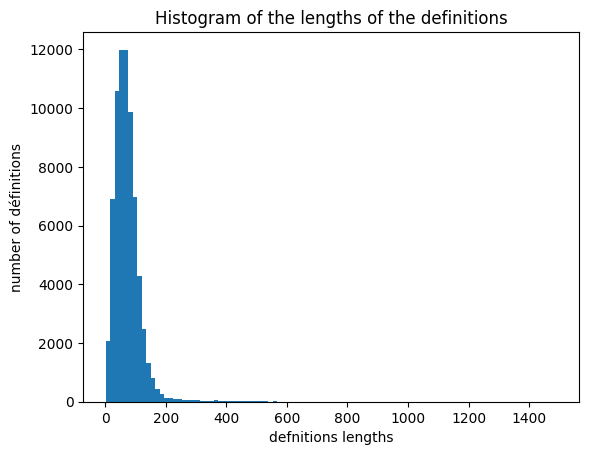
\includegraphics[width=0.7\textwidth]{img/lengths.png}
    \caption{Histogramme de la répartition des longueurs de définitions}
    \label{fig:lengths}
\end{figure}

\subsection{Entraînement}

L'entraînement est réalisé en une seule époque (ou plus si on réentraîne le modèle ultérieurement). La taille du batch est de 8 pour éviter la surchage mémoire des GPU.

Pour le modèle GPT-2, le temps total d'entraînement est d'environ 1h.

\subsection{Utilisation du modèle}

Comme lors du TP5, nous utilisons ici la fonction \texttt{pipeline} de la librairie Transformers pour générer le texte. Le modèle est chargé avec le tokenizer associé.

Le modèle étant entraîné sur des exemples de la forme \texttt{Define: \textless mot\textgreater\textbackslash n\textless definition\textgreater}, il faut donc préparer le prompt d'entrée (listing \ref{listing:generate}).

\begin{listing}[H]
    \begin{minted}[breaklines,bgcolor=LightGray]{python}
def generate(prompt, numDef):
    fullPrompt = f"Define: {prompt}\n"
    results = generator(fullPrompt, num_return_sequences=numDef, ...)
    return [result["generated_text"] for result in results]

for result in generate("zoophobia", 3):
    print(result, end="\n\n")
    \end{minted}
    \caption{Fonction de génération de texte}
    \label{listing:generate}
\end{listing}

\section{Analyse des résultats}

En commençant ce projet nous espérions que le modèle apprenne à reconnaitre des préfixes, suffixes et radicaux et à les associer à un sens précis. Cette appproche est parfaitement en accord avec la notion de jetons que le modèle de langage utilise pour générer du texte.

Malheureusement, le fait de patir d'un modèle préentraîné impose le tokeniser et notre affinage ne permet pas de le modifier. Il faut donc se contenter du tokeniseur du modèle de base.

\subsection{Modèle non affiné}

% TODO: 2-3 examples

\subsection{Modèle affiné}

% TODO: essayer plein de defs et analyser

\section{Conclusion}

% TODO

\end{document}